\section{Pokémon Platinum Definition's}

The game itself, paired with online community driven sources, provide all the necesarry information to define pokémon's in a mathimatical fashion.

\subsection{Types}

% Reasoning for choosing a tuple and not a set is that later on, being able to reference types by numbers becomes important during programming. To reference a type by a number means ordering is important, thus the choice for a tuple over a set.

The \emph{Types} $T$ is a constant 18-tuple containing the following strings:
\begin{itemize}
    \item $T_0$  = none
    \item $T_1$  = normal
    \item $T_2$  = fire
    \item $T_3$  = water
    \item $T_4$  = electric
    \item $T_5$  = grass
    \item $T_6$  = ice
    \item $T_7$  = fighting
    \item $T_8$  = poison
    \item $T_9$  = ground
    \item $T_{10}$ = flying
    \item $T_{11}$ = psychic
    \item $T_{12}$ = bug
    \item $T_{13}$ = rock
    \item $T_{14}$ = ghost
    \item $T_{15}$ = dragon
    \item $T_{16}$ = dark
    \item $T_{17}$ = steel
\end{itemize}

\subsection{Moves}

A singular \emph{move} $m$ is a 7-tuple $(\text{name}, \text{type}, \text{category}, \text{power}, \text{accuracy}, \text{pp}, \text{effect})$, where:
\begin{itemize}
    \item name is the name of the move as a string.
    \item type $\in T$ is the type of the move.
    \item category $\in \{ \text{physical}, \text{special}, \text{status}, \lambda \}$ is the category of the move.
    \item power $\in \mathbb{N}$ is the power of the move.
    \item accuracy $\in \mathbb{N}$ is the accuracy of the move.
    \item pp $\in \mathbb{N}$ is the power points of the move.
    \item effect is the effect of the move as a string.
\end{itemize}

\paragraph{}
The set of moves $\mathbb{M}$ in Pokémon Platinum is constant and known beforehand. A list of all moves can be found at \href{http://www.psypokes.com/dpphgss/attacks.php}{Psypokes}.

\paragraph{}
The empty move $m \in \mathbb{M}$ is defined as $(\lambda, T_0, \lambda, 0, 0, 0, \lambda)$

\subsection{Abilities}

\emph{Abilities} $\mathbb{A}$ is a set of all abilities. A list of all abilities can be found at [Psypokes](http://www.psypokes.com/dpphgss/abilities.php).

TODO: Research if abilities are constant or if they can change during the game.  
TODO: Research different types of abilities and define functions that can be used to determine if an ability is of a certain type.

\subsection{Items}

\emph{Items} $\mathbb{I}$ is a set of all items available in Pokémon Platinum. A list of all items can be found at [Serebii.net](https://www.serebii.net/platinum/items.shtml).

An item $x \in \mathbb{I}$ is a 3-tuple $(name, function, type)$, where:
\begin{itemize}
    \item $name$ is the name of the item as a string.
    \item $function$ is the function $f$ of item $x$ such that when used, $f$ either does or does not result in a state change.
    \item $type$ is the type of the item.
    \begin{itemize}
        \item $type \in \{ \text{healing} \}$ dictates the change in state of item $x$.
    \end{itemize}
\end{itemize}

\subsection{Bag}

The bag $\mathbb{B}$ is the set of items available to any given agent in state $s$.

\subsection{Status Effects}

Status effects $\mathbb{E}$ is a 5-tuple $( \text{poisoned}, \text{burned}, \text{paralyzed}, \text{asleep}, \text{frozen} )$.
TODO: Describe each effect in detail.

\subsection{Nature}

TODO: define pokemon natures mathimatically

\subsection{Pokémon}

A \emph{Pokémon} $p \in \mathbb{P}$ is a ...-tuple $( 
    \text{base hp}, \text{base atk}, \text{base def}, \text{base spatk}, \text{base spdef}, \text{base spd}, \break
    \text{hp iv}, \text{atk iv}, \text{def iv}, \text{spatk iv}, \text{spdef iv}, \text{spd iv}, 
    \text{hp ev}, \text{atk ev}, \text{def ev}, \text{spatk ev}, \text{spdef ev}, \text{spd ev}, \break
    \text{level}, \text{ability}, \text{nature}, t_1, t_2, m_1, m_2, m_3, m_4, \text{status}
    )$, where:
\begin{itemize}
    \item $\mathbb{P}$ is the set of all Pokémon available in Pokémon Platinum. It is constant and known beforehand. A list of Pokémon can be found at [TODO: add link to the Pokémon Platinum Dex](lin).
    \item $hp, \text{atk}, \text{def}, \text{spatk}, \text{spdef}, \text{spd} \in \mathbb{N}$ are the Pokémon's stats, those being: hit points, physical attack power, physical defensive power, special attack power, special defensive power, and speed, respectively.
    \begin{itemize}
        \item TODO: Describe that stats are all functions, such that:
            \begin{itemize}
                \item $hp(p) = \left[ \frac{2 \times \text{base} + \text{iv} + (\frac{\text{ev}}{4}) \times \text{level}}{100} \right] + level + 10$
                \item All other stats $f(p) = \left[ \left( \left[ \frac{2 \times \text{base } + \text{ iv} + (\frac{\text{ ev}}{4}) \times \text{level}}{100} \right] + 5 \right) \times \text{nature} \right]$
            \end{itemize}
    \end{itemize}
    \item $iv \in \mathbb{N}$ is the Pokémon's individual value.
    \item $ev \in \mathbb{N}$ is the Pokémon's effort value, which are bonus stats that can be gained through battling.
    \item ability $x \in \mathbb{A}$.
    \item $t_1, t_2 \in T$ are the Pokémon's types.
    \begin{itemize}
        \item $monotype$ is a function on $p$ that results in a boolean value. A Pokémon $p$ is considered to be monotype if $p_{t_2} = T_0$, and dual type otherwise.
        \item $partialtype$ is a function on $p$ that results in a boolean value. A Pokémon $p$ is considered to be partialtype if $p_{t_1} = T_i \lor p_{t_2} = T_i$.
    \end{itemize}
    \item $m_1, m_2, m_3, m_4 \in \mathbb{M}$ are the Pokémon's moves.
    \item $status \in \mathbb{E}$.
\end{itemize}

\subsection{Pokémon Party}

A Pokémon party is a 6-tuple $(p_1, p_2, p_3, p_4, p_5, p_6)$ where $p \in \mathbb{P}$.

\subsection{Effectiveness}

The effectiveness of a move $m$ against a Pokémon $p$ is a function $E(m, p) \in \{0, 0.5, 1, 2, 4\}$, where:
\begin{itemize}
    \item The value is dictated by the type chart $C$, which is an 18x18 matrix where $C_{i, j}$ is the effectiveness of type $T_i$ against type $T_j$.
    \item The value of effectiveness is compared to both of $p$'s types and added together.
    \item For example:
    \begin{itemize}
        \item If $p_{t_1} = \text{grass}$, $p_{t_2} = \text{ice}$ and $m_t = \text{fire}$, then $E(m, p) = C_{m_t, p_{t_1}} + C_{m_t, p_{t_2}} = C_{2, 5} + C_{2, 6} = 2 + 2 = 4$.
    \end{itemize}
\end{itemize}

% \begin{figure}[h!]
%     \centering
%     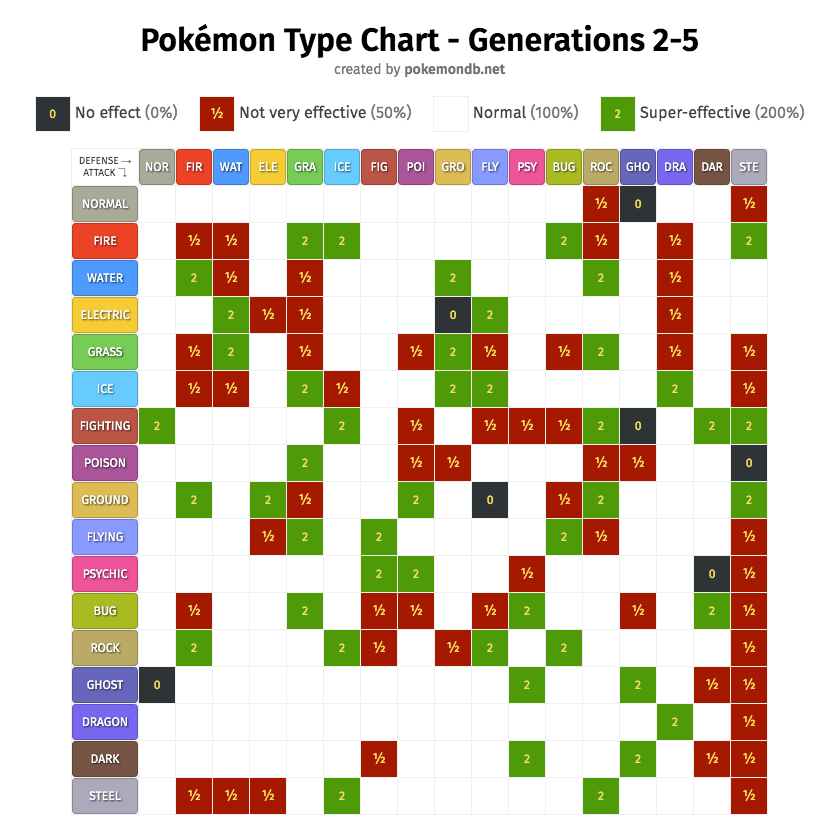
\includegraphics[width=0.8\textwidth]{https://img.pokemondb.net/images/typechart-gen2345.png}
%     \caption{A visual representation of the Generation 4 type chart as provided by [pokemondb.net](https://pokemondb.net/type/old).}
%     \label{fig:typechart}
% \end{figure}